\section{VALIDACIÓN DE RESULTADOS}

Como proyecto de ingeniería, se debe llevar a cabo un análisis de cumplimiento de los requerimientos del sistema desarrollado a través de métricas. Para la validación se van a evaluar las 
diferentes partes del trabajo.

Primeramente, a través del entrenamiento de la red neuronal, se ha buscado minimizar el error asociado a las \texttt{Bounding Boxes}, ya que el sistema usa esto como base para calcular movimientos. 
En este sentido, con el último conjunto de datos y 600 épocas, se han conseguido alcanzar un error de \texttt{0.2} y \texttt{0.9} en el conjunto de datos de entrenamiento y validación respectivamente, siendo 
este resultado uno de los mejores de todos los entrenamientos y con un conjunto de validación mucho más realista. Los resultados de la validación se pueden ver en la \autoref{fig:ValidacionRed}.

\begin{figure}[H]
    \centering
    \begin{subfigure}[b]{0.7\textwidth}
        \centering
        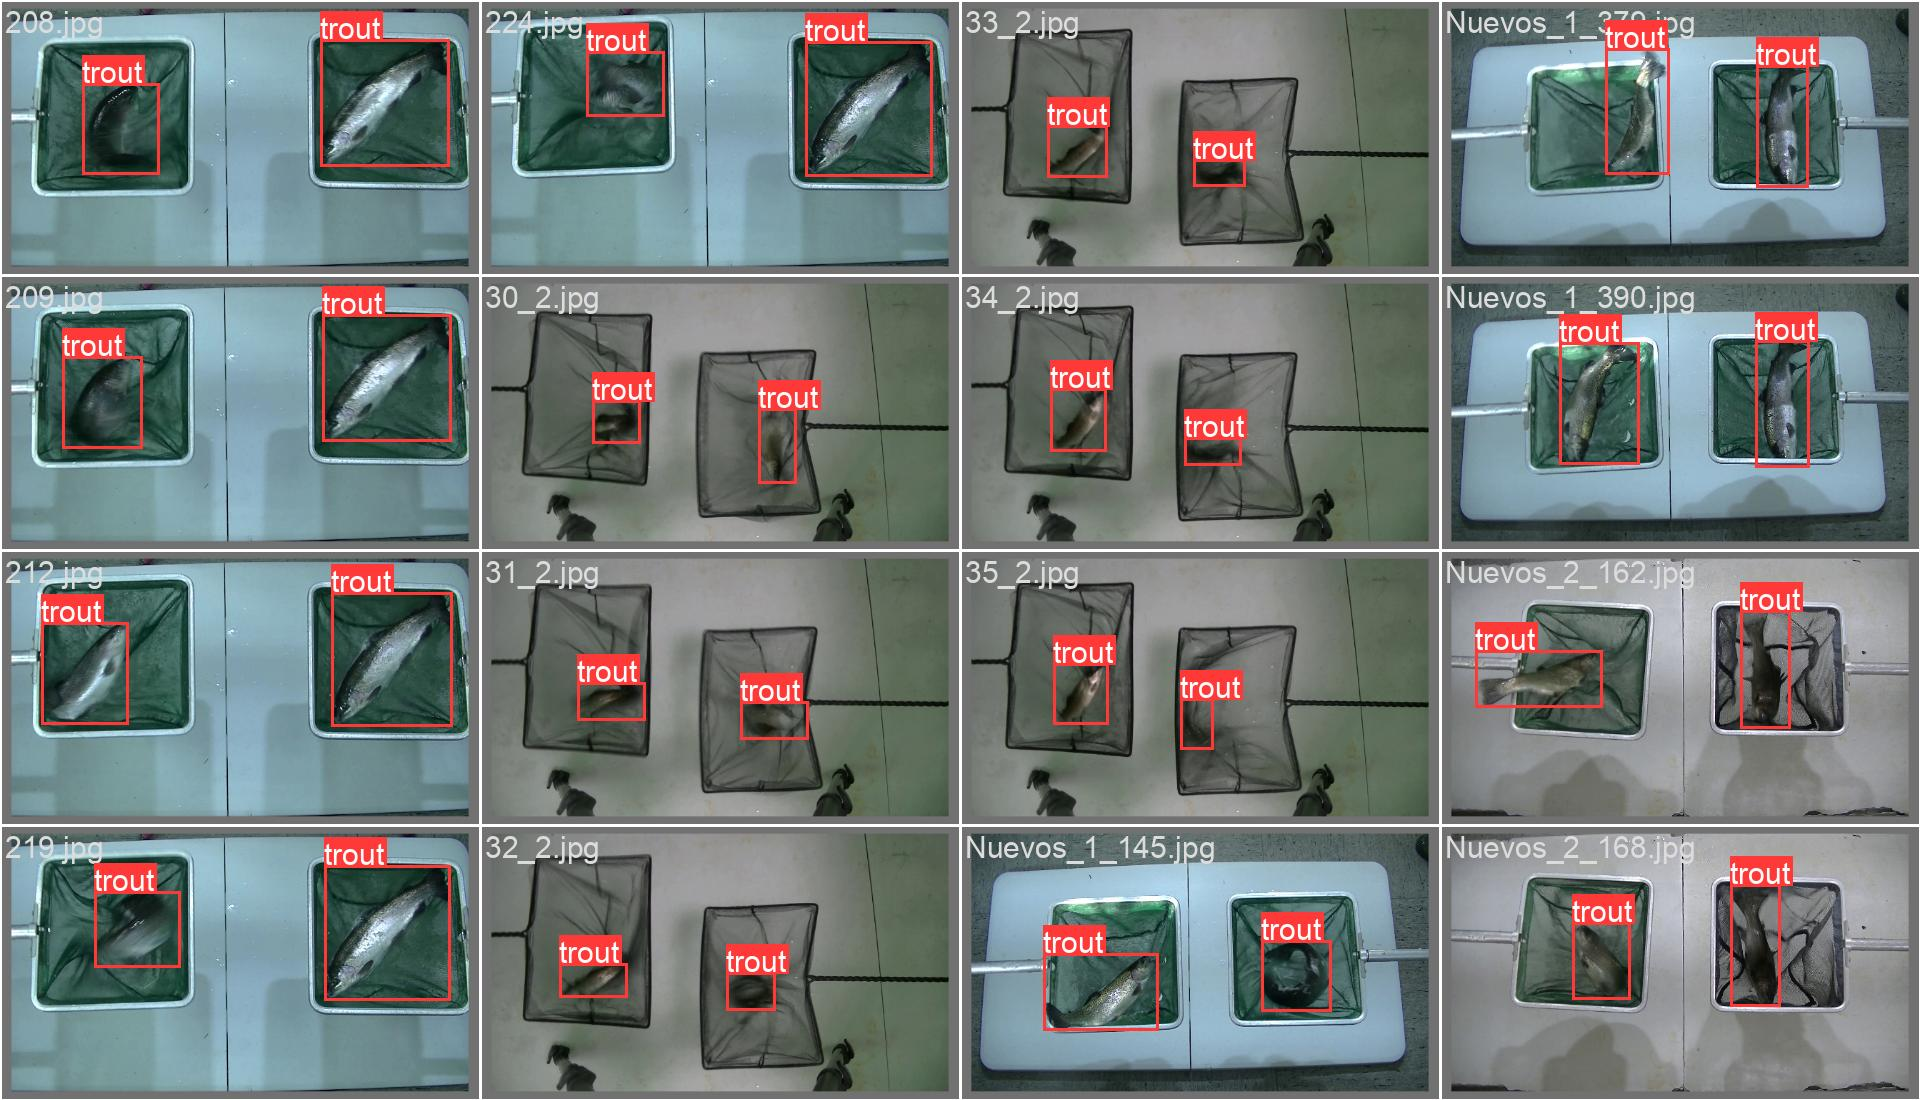
\includegraphics[width=0.95\textwidth]{images/7/labels.jpg}
        \caption{Etiquetas del conjunto de validación final}
    \end{subfigure}
    \begin{subfigure}[b]{0.7\textwidth}
        \centering
        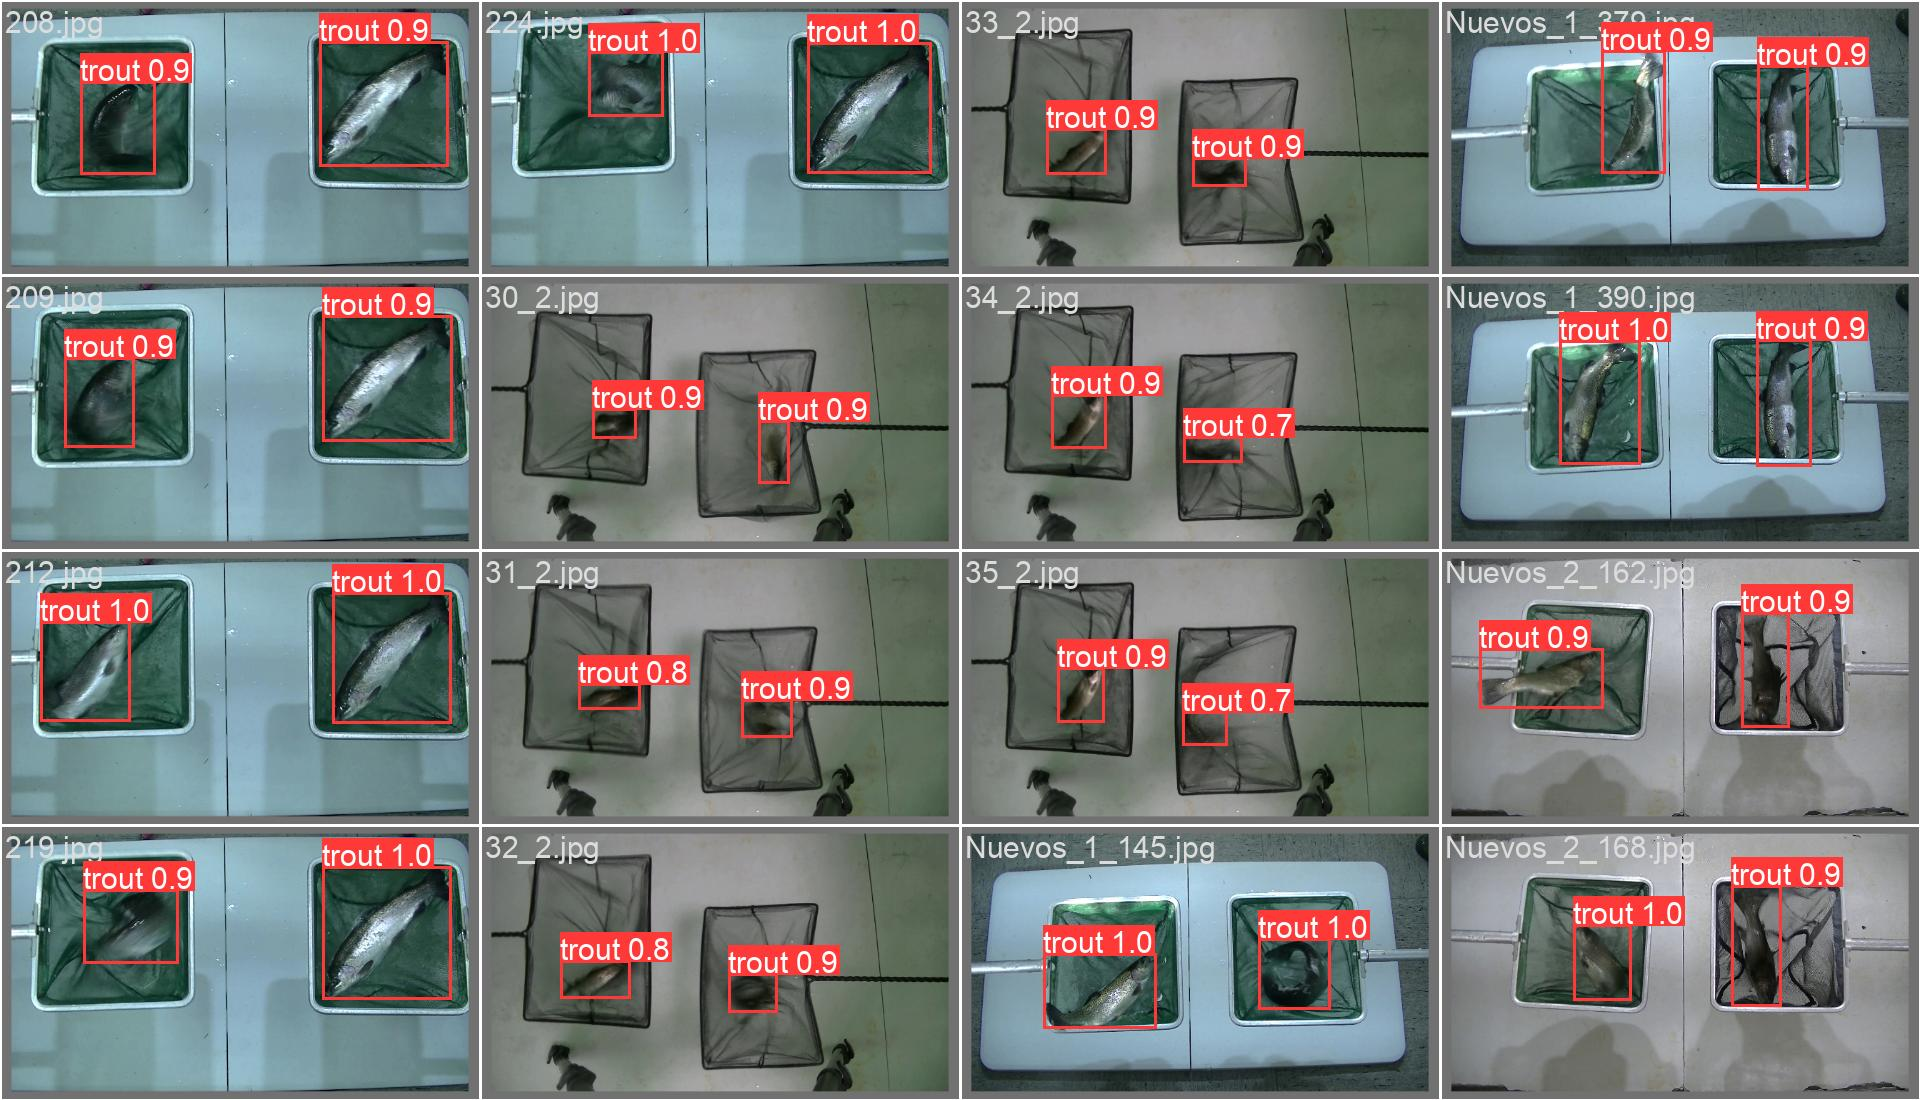
\includegraphics[width=0.95\textwidth]{images/7/pred.jpg}
        \caption{Predicciones sobre el conjunto de validación final}
    \end{subfigure}
    \caption{Resultados finales sobre el conjunto de validación}
    \label{fig:ValidacionRed}
\end{figure}

Aparte de los resultados de validación, como ya se ha dicho en el trabajo y se puede ver en \hyperref[train:final]{las gráficas de resultados del anexo c}, se buscaba maximizar otras métricas como son 
el \texttt{recall} a niveles altos para obtener una cantidad elevada de verdaderos 
positivos. Finalmente, también se ha conseguido alcanzar una precisión \texttt{mAP50-95} muy elevada (0.82) teniendo en cuenta la variabilidad del conjunto de datos, lo cual nos indica una precisión 
general de la red muy buena.

\clearpage

Seguidamente, para validar el número de movimientos de la aplicación contra los reales se tuvo en cuenta que la estimación de las etiquetas proporcionadas por los investigadores tenían demasiados errores, ya que 
no usaban siempre la misma definición de movimiento.

Para esta validación, se ha definido movimiento como la compresión realizada por la trucha antes de estirarse (es cuando la \texttt{Bounding Box}) tiene menor área.

Se ha realizado una validación con 50 videos aleatorios de todo el conjunto de videos, excluyendo los videos usados para el entrenamiento de la res, que son: \verb|23_NT_R1_J1_P1_2|, \verb|23_NT_R2_J1_P1_P2|, \verb|23_NT_R3_J1_P1_P2| 
y \verb|23_NT_R3_J2_P1_P2|. Los resultados se pueden ver en la , en la cual aparecen el valor del número de movimientos asignado por los científicos solo por comparativa, ya que por lo comentado anteriormente, no es riguroso.